\chapter{Background \& Objectives}

\section{Problem Description}

The Travelling Salesperson Problem (TSP) is an NP-Hard problem\cite{BASSETTO2011253} and is tasked with solving the problem "Given a list of cities and the distances between each city what is the shortest possible route that visits each city once and then returns to the origin city". This shortest route is called a Hamiltonian Cycle and has many applications such as in the fields of logistics, route planning and manufacturing. 

My project is a way of solving TSPs with the use of clustering and an Ant Colony Optimisation (ACO) Algorithm. ACO is a probabilistic technique that is based off how ants work in nature, figure \ref{fig:aco_pheremone_example} shows an example of how the path of ants change as pheromone gets deposited.

\begin{figure}
    \centering
    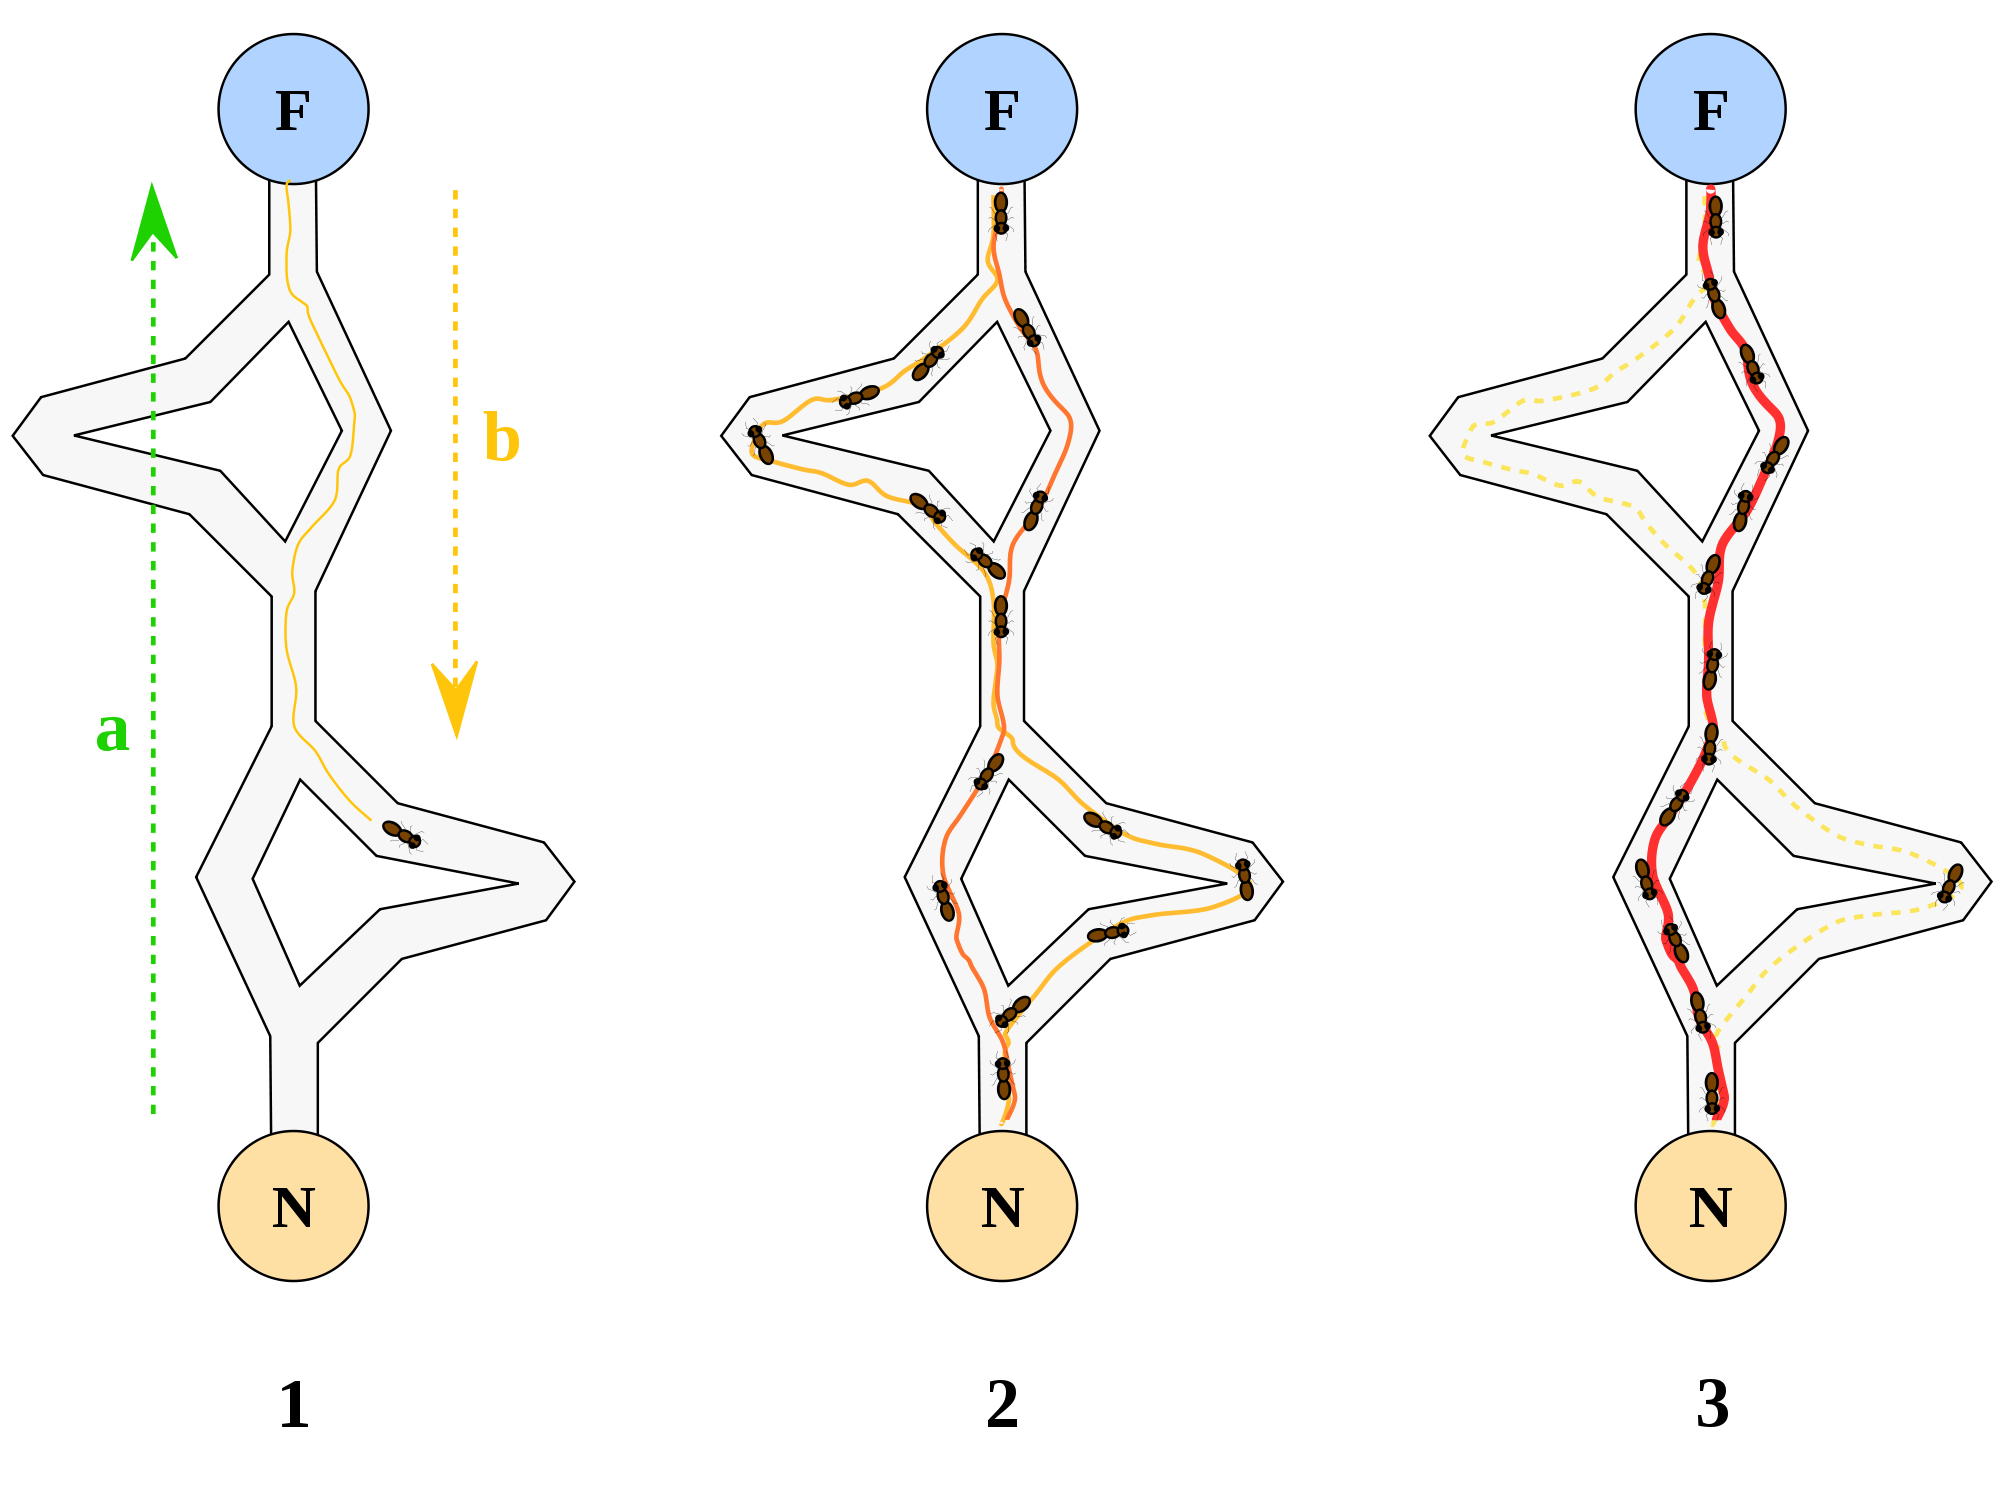
\includegraphics[width=\textwidth]{Project Report/LaTeX Template/figures/aco_pheremone_demo.png}
    \caption{Figure showing how in nature ants deposit pheromone and change their paths based on the pheremone from other ants.}
    \label{fig:aco_pheremone_example}
\end{figure}

There are many freely available data sets of TSPs\cite{tsp_test_data_2009} these are all of varying sizes and complexity, they also all have their optimal solutions noted so that easy comparisons can be made and so I can see how my algorithm performs. 

\section{Background}
My motivation for this project was based around my interest in Algorithms and finding new approaches to solve challenging problems, TSPs have been widely studied with many algorithms having been made to solve them. 

In 1991 ACO was first applied to solve TSPs\cite{dorigo1991distributed}, ACO is well suited to solve optimisation problems because it can relatively quickly compute lots of solutions and can quickly remove bad solutions. ACO is not efficient at finding the solution for large problems because its run time is to high, it's possible to tune the parameters of the algorithm such as reducing the number of iterations it will perform however doing this could mean that it finds a worse solution, because ACO is probabilistic it's possible for it to find different solutions to the same problem on consecutive runs. 

\section{Analysis}
**Taking into account the problem and what you learned from the background work, what was your analysis of the problem? How did your analysis help to decompose the problem into the main tasks that you would undertake? Were there alternative approaches? Why did you choose one approach compared to the alternatives? 

There should be a clear statement of the research questions, which you will evaluate at the end of the work. 

In most cases, the agreed objectives or requirements will be the result of a compromise between what would ideally have been produced and what was felt to be possible in the time available. A discussion of the process of arriving at the final list is usually appropriate.**

Questions:

Does applying clustering help to speed up the ACO process

What effect does the clustering algorithm, parameters and ACO parameters effect the run time and the quality of the solution

\section{Software Process}
You need to describe briefly the life cycle model or research method that you used. You do not need to write about all of the different process models that you are aware of. Focus on the process model or research method that you have used. It is possible that you needed to adapt an existing method to suit your project; clearly identify what you used and how you adapted it for your needs.

For the research-oriented projects, there needs to be a suitable process for the construction of the software elements that support your work.
